\documentclass[12pt]{article}
\usepackage[a4paper, margin=.30in]{geometry}
\usepackage{graphicx ,
            wrapfig,
            xcolor, 
            enumerate,
            amsmath,fontenc, mhchem
            }

\newcommand\headerMe[2]{\noindent{}#1\hfill#2}
\renewcommand{\thesection}{\Roman{section}}

\author{Zakaria HAOUZAN}
\date{\today}

\begin{document}
% headers --------------
\headerMe{Matière : Physique-Chimie}{Professeur : Zakaria HAOUZAN}\\
\headerMe{Unité : Travail Mécanique et Energie }{Établissement : Lycée SKHOR qualifiant}\\
\headerMe{Niveau : 1BAC-SM-X}{Heure : 6H}\\

% ------Content ________
\begin{center}

    \Large{Leçon $N^{\circ} 6 $: \color{red}Les réactions acido-basiques  }
\end{center}

%\begin{wrapfigure}[10]{r}{0.5\textwidth}
%    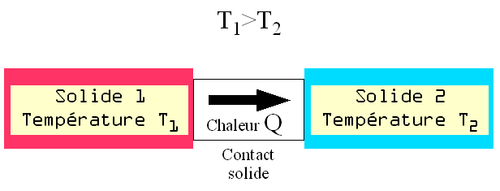
\includegraphics[width=0.5\textwidth]{./img/img00.png}
%\end{wrapfigure}
\section{Notion d’acide et base selon de Bronsted : }
\subsection{ Exemple de réaction acido-basique :}
\begin{itemize}
      \item Réaction entre l’acide nitrique et l’eau : 
         \\La réaction entre l’acide nitrique $HNO_3$ et l’eau produit des ions nitrate $NO_3^-$ et des ions oxonium $H_3O^+$selon la réaction suivante $${HNO_3}_{(l)} + {H_2O}_{(l)} \rightarrow {NO_3^-}_{aq} + {H_3O^+}_{(aq)}$$
         \item On constate au cours de cette équation que l’espèce chimique $HNO_3$ a perdu un proton $H^+$ alors que l’espèce $H_2O$ a gagné ce proton.

\end{itemize}
\subsection{Définition de l’acide et de base selon Bronsted : }
On appelle acide une espèce chimique capable de céder un ou plusieurs protons $H^+$.

Exemple : $H_2O ; H_3O^+ ; NH_4^+; HCOOH$.

On appelle base une espèce chimique capable de capter un ou plusieurs protons $H^+$
$HO^{-} ; H_2O ; NH_3 ; HCOO^-$


\section{Couples acide / base :}


Deux espèces chimiques constituent un couple acide / base s’il est possible de passer
de l’un à l’autre par perte ou gain d’un proton $H^+$.

Exemples : acide/base $NH_4^+/NH_3 \ ; H_2O/HO^-  ; H_3O^+/H_2O$

\subsection{Demi-équation acido-basique :}
Soit $AH/A^-$ un couple acide/base.
\begin{itemize}
   \item Si AH est l’un des réactifs il va donner sa base conjuguée : $AH \rightarrow A^- + H^+$
   \item Si $A^-$ est l’un des réactifs il va donner son acide conjugué : $A^- + H^+ \rightarrow AH$
   \item La demi-équation du couple acide/base $AH/A^-$ s’écrit :$$AH \rightleftharpoons A^- + H^+ $$
\end{itemize}
Exemple : \ce{$\underset{\text{ion ammonium}}{\ce{NH4+}}$ <=>$\underset{\text{ammoniac }}{\ce{NH3}} + \ce{H+}$ } 
\subsection{ Couple acide- base de l’eau : }
L’eau a des propriétés acido-basiques :

*c’est un acide : \ce{H2O <=>$\underset{\text{Ion hydroxyde }}{\ce{HO-}} + \ce{H+}$} *c’est une base :\ce{$\underset{\text{ion oxonium}}{\ce{H3O+}}$ <=> \ce{H2O} + \ce{H+}}
\subsection{Notion d’ampholyte : }
L’eau se comporte comme un acide dans le couple \ce{H2O/HO-}et comme une base dans le couple \ce{H3O/H2O}, on l’appelle ampholyte (ou amphotère).

\section{L’équation chimique d’une réaction acido-basique :}
Si l’acide $A_1H$ réagit avec la base $A_2^-$, On écrit directement les demi-équations dans le sens où elles se produisent.$$\ce{A1H <=> A1- + H+}$$ $$\ce{A2- + H+ <=> A2H}$$
La combinaison de ces 2 demi-équations donne l’équation de la réaction :
$$\ce{A1H + A2- <=> A1- + A2H}$$

\subsection{Application 1 :}
La base $NH_3$ réagit avec l’acide éthanoïque CH3COOH.
1- Ecrire les couples qui participent dans cette réaction.
2- Ecrire l’équation de la réaction.

\section{Indicateurs colorés acido-basiques : }
Un indicateur coloré est un couple acide-base dont l’acide HIn et la base $In^-$ n’ont pas la même couleur. Son couple est noté : $HIn/In^-$

En présence de l’acide HA, la base de l’indicateur réagit selon la réaction :
$$\ce{In- + HA -> HIn + A-}$$

Le mélange prend la couleur de l’espèce acide HIn.

En présence de la base $A^-$, l’acide de l’indicateur réagit selon la réaction :
$$\ce{HIn + A- -> In^- + HA}$$
Le mélange prend la couleur de l’espèce basique $In^-$.

\begin{center}
   \begin{tabular}{|c|c|c|}
      \hline
      Indicateur coloré & Couleur de l’espèce acide & Couleur de l’espèce base\\\hline
      BBT               & Jaune                     & Bleue\\\hline
      Hélianthine       &Rose                       & Jaune\\\hline
      Phénolphtaléine   & inclore                   & rose \\\hline
   \end{tabular}
\end{center}

\subsection{Exemples de couple acido-basique : }

\begin{center}
   \begin{tabular}{|c|c|c|c|}
      \hline
      demi-équation                  & L’acide &sa base conjuguée &couple acido-basique  \\\hline
      \ce{CH3COOH <=> CH3COO- + H+ } &         &                  & \\\hline
                                     &         &                  & \ce{HNO3/NO3-}\\\hline
                                     &         &                  & \ce{NH4+/NH3}\\\hline
      \end{tabular}
\end{center}
\subsection{Application 2 :}
1- Ecrire les demi-équations de réactions acido-basiques relatives à :

a- L’acide nitreux \ce{HNO2_(aq)}

b- L’ammoniac \ce{NH3 (aq)}

2- En déduire l’équation de la réaction entre l’acide nitreux et l’ammonic.
\section{Exercice : }

On mélange un volume V1 = 12,0 mL d’une solution d’acide méthanoïque \ce{HCOOH(aq)}
de concentration $C_1$=0,16 mol/L avec un volume $V_2$ = 23,0 mL d’une solution basique
de l’ammoniac \ce{NH3 (aq)} de concentration $C_2 = 5 × 10^{-3}mol/L$.

1- Avec quelle verrerie a-t-on pu mesurer les volumes indiqués ?

Pipettes graduées de 25 mL ou burette de 25 mL

2- Ecrire les couples acide/base étudiés et la demi-équation de chaque couple.
3- Ecrire l’équation de la réaction qui peut se produire.
4- Etablir la composition finale du système en quantité de matière, puis en
concentrations (construire le tableau d’avancement).
\end{document}

